% Plan 9
\documentclass[12pt,UTF8]{ctexbook}

\input{../../../Book/common/page}

% 设置字体，并解决显示难检字问题。
\xeCJKsetup{AutoFallBack=true}
\setCJKfamilyfont{hei}{SimHei}
\setCJKfamilyfont{kai}{KaiTi}

% 目录 chapter 级别加点（.）。
\usepackage{titletoc}
\titlecontents{chapter}[0pt]{\vspace{3mm}\bf\addvspace{2pt}\filright}{\contentspush{\thecontentslabel\hspace{0.8em}}}{}{\titlerule*[8pt]{.}\contentspage}

% 支持目录点击跳转
\usepackage[colorlinks,linkcolor=blue,citecolor=blue,urlcolor=blue]{hyperref}

% 设置 part 和 chapter 标题格式。
\ctexset{
	part/name= {第,卷},
	part/number={\chinese{part}},
	chapter/name={第,篇},
	chapter/number={\arabic{chapter}}
}

% 图片相关设置。
\usepackage{graphicx}
\graphicspath{{Images/}}

\usepackage{float}

% 设置署名格式。
\newenvironment{shuming}{\hfill\zihao{4}}

% 注脚每页重新编号，避免编号过大。
\usepackage[perpage]{footmisc}

% 设置段落间距
\setlength{\parskip}{0.8em plus 0.2em minus 0.1em}

% 列表格式支持，列表项向右偏移。
\usepackage{enumitem}

% 表格支持
\usepackage{longtable, booktabs}

\title{\heiti\zihao{0} Plan 9 from Bell Labs}
\author{}
\date{}

\begin{document}
	
\maketitle
\tableofcontents
	
\frontmatter

\chapter{序言：为何学习 Plan 9}
	
Plan 9 from Bell Labs 是由贝尔实验室计算科学研究中心于 1980 年代中期至 2002 年开发的分布式操作系统。它由 Unix 创造者 Ken Thompson、Rob Pike、Dave Presotto 和 Phil Winterbottom 等人设计，旨在成为 Unix 的精神继任者。在随后的十年中，众多研究者加入了开发行列。
	
Plan 9 展示了一种全新且通常更为简洁的方法来解决大多数系统问题。对于 Unix 用户而言，整个系统可能会让人感到既熟悉又陌生。
	
Plan 9 的核心设计理念可概括为三大支柱：

\begin{enumerate}
\item \textbf{一切皆是文件}：所有系统资源（CPU、内存、网络、进程等）均以文件形式呈现，比 Unix 更加彻底。
\item \textbf{统一的 9P 协议}：内核只认识 9P 这一种协议，所有资源访问均通过标准化的消息传递完成。该连接可以是网络连接、管道或任何其他可读写且另一端运行着 9P 服务器的文件描述符。
\item \textbf{私有可塑的命名空间}：每个进程拥有自己独立的文件视图，可通过 \texttt{bind}、\texttt{mount} 等命令自由定制，且不会影响其他不相关进程的命名空间。
\end{enumerate}

在 Plan 9 中，每个进程都有自己的可变命名空间。一个进程可以重新排列、增加或删除自己的命名空间，而不会影响无关进程的命名空间。命名空间变更中包括挂载到遵循 9P 协议的文件服务器连接的能力，9P 是一种简单的文件协议。该连接可以是网络连接、管道，或任何其他打开用于读写的文件描述符，另一端是 9P 服务器。
	
定制化的命名空间在整个系统中被广泛使用，用于呈现新资源（如窗口系统）、从另一台机器导入资源（如网络栈）或向后浏览历史版本（例如转储文件系统）。
	
Plan 9 不仅是一个操作系统内核，更是一套完整的配套软件集合。其大部分软件都是全新编写的，专门为 Plan 9 设计而非从 Unix 或其他系统移植而来。窗口系统、编译器、文件服务器和网络服务均为 Plan 9 重新编写。尽管经典的 Unix 程序如 \texttt{dc(1)}、\texttt{ed(1)} 乃至 \texttt{troff(1)} 也被引入，但它们通常以更新的形式存在——例如，troff 接受以 UTF-8 编码的 Unicode 文档，与系统的其他部分保持一致。
	
本框架将 Plan 9 的学习路径划分为 \textbf{六卷、二十二篇文章}，涵盖从设计哲学、日常使用、内核源码到云计算生态的完整知识体系。建议学习者循序渐进，并时刻铭记：\textbf{在 Plan 9 中，如果它看起来不像文件，那一定是你还没找到正确的挂载点。}
	
~\\

\begin{shuming}
WangFei \hspace{2em} \today
\end{shuming}
	
\mainmatter
	
% ============================================================
% 第一卷：基础与哲学
% ============================================================

\part{基础与设计哲学}
	
\chapter{历史渊源、版本演进与设计决策}

理解 Plan 9 的设计哲学，不能脱离其诞生的历史语境。本章将带领读者穿越从 1980 年代初期构想到 2021 年 MIT 开源的完整历程，揭示那些塑造了 Plan 9 独特面貌的关键决策。

我们首先回顾 Plan 9 的诞生背景——为何 Unix 的创造者们会感到不满，进而萌生另起炉灶的念头。随后，我们将追踪系统从早期实验到四个主要版本发布的技术演进，剖析每一个版本背后的设计权衡。最后，本章将归纳 Plan 9 的三大核心设计原则，并简要评述其对后世操作系统和编程语言的影响。

对于初次接触 Plan 9 的学习者而言，本章提供了一幅宏观的历史地图；对于已有 Unix 经验的技术人员，本章则揭示了 Plan 9 何以被称为“Unix 的精神继任者”而非简单变体的根本原因。

\section{Plan 9 的诞生背景}

Plan 9 是贝尔实验室开发的一个研究型系统，始于 20 世纪 80 年代末，旨在摆脱 Unix 时代“众多独立工作站各自为政”的碎片化困境，构建一个集中管理、经济高效的系统。其设计初衷是：将计算资源（CPU、存储、网络）与用户界面分离，通过统一的协议进行透明访问。
	
最初的设计者和作者是 Ken Thompson（肯·汤普森）、Rob Pike（罗伯·派克）、Dave Presotto（戴夫·普雷索托）和 Phil Winterbottom（菲尔·温特伯顿），随后在 1990 年代至今的持续开发中，众多其他研究者加入其中。

\section{从构想到启动：设计理念的早期酝酿}

在正式发布之前，Plan 9 经历了长达数年的构思与早期实验阶段。

\subsection{1984 年的最初构想}

1984 年左右，Ken Thompson 和 Rob Pike 已经开始思考如何摆脱 Unix 日益增长的复杂性。Unix 的成功带来了大量的新特性，但也使得系统变得臃肿。Thompson 和 Pike 认为，真正的解决方案不是修补 Unix，而是重新设计一个更简洁、更统一的系统。

\subsection{1989 年初：硬件订单与项目启动}

1989 年初，贝尔实验室的团队订购了专用硬件，开始搭建 WORM（Write-Once, Read-Many）文件服务器和内核原型。这是 Plan 9 作为正式项目的起点。

\subsection{1989 年秋：关键突破}

1989 年秋天，在一次晚餐后的讨论中，Thompson 和 Pike 意识到系统需要一个关键的架构改进：能够挂载用户空间文件描述符，而不仅仅是网络地址。这一认识催生了一系列核心机制的诞生：

\begin{itemize}
\item \texttt{bind} 系统调用——用于重新排列命名空间
\item 新的 \texttt{mount} 机制——支持任意文件描述符的挂载
\item \texttt{flush} 机制——用于处理 I/O 取消
\end{itemize}

经过几天的重构，他们让整个系统重新运转起来。此时设计的协议与最终发表的 9P 协议在本质上已经基本一致。

\subsection{1990 年：自托管与内部推广}

\begin{itemize}
\item \textbf{1990 年 5 月}：系统尝试自托管（self-hosting），文件服务器和窗口系统经历了多次重写，但已有十多位内部用户开始使用。
\item \textbf{1990 年 7 月}：团队向 UKUUG（英国 Unix 用户组）提交了著名的论文 \textit{Plan 9 from Bell Labs}，首次将这一系统公之于众。
\end{itemize}
	
\section{版本演进历史}
	
Plan 9 在其生命周期中经历了四个主要版本。
	
\subsection{第一版（1992 年）}

\begin{itemize}
\item 仅面向大学发布。
\item 包含 Plan 9 的大部分可识别部件：内核、\texttt{ndb}、\texttt{sam}、\texttt{upas}、\texttt{alef} 语言以及完整的 UTF-8 支持。
\item \texttt{Acme} 以早期形式作为 \texttt{help} 存在。
\item CPU 服务器为 Sun Sparcstation、SGI Power 和 SGI Magnum，终端为 NeXTstations 和 PC。
\item 本地构建的 Gnot 和 Hobbit 工作站也被用作终端。
\end{itemize}
	
\subsection{第二版（1995 年）}

\begin{itemize}
\item 以书籍附赠 CD-ROM 的形式发布。
\item 新增了 \texttt{acme} 和一些较小的实用工具。
\item 此时 Plan 9 团队已在开发一个名为 \textbf{Brazil} 的系统重构版本。
\item 1999 年，为迎接第三版发布，Brazil 的名称被恢复为 Plan 9。
\end{itemize}

\subsection{第三版（2000 年 6 月）}

\begin{itemize}
\item 通过互联网免费发布。
\item 引入了新的彩色图形操作符 \texttt{draw} 和新的程序连接机制 \texttt{plumbing}。
\item 引入了名为 \texttt{wrap} 的简单更新管理器，用于安装打包的系统更新。
\item 第三版发布后不久，贝尔实验室团队开始了对 9P 协议的修订\footnote{移除了对文件名长度的一些繁琐限制。在目录元数据中添加了“最后修改者”（last modifier）字段。批量处理 walk 消息。引入认证文件作为将认证协议细节移出 9P 协议本身的一种机制。}，称为 \textbf{9P2000}。
\end{itemize}
	
\subsection{第四版（2002 年）}

\begin{itemize}
\item 引入了 9P2000 协议。
\item 新增了相关的安全代理 \texttt{factotum(4)} 和密钥存储 \texttt{secstore(8)}。
\item 引入了 \texttt{venti(8)} 块存储服务器。
\item 基于 Venti 的文件服务器 \texttt{fossil(4)} 于 2003 年初首次亮相。
\item 引入了新的系统更新分发机制：公共 fossil 文件服务器 \texttt{sources.cs.bell-labs.com} 持有当前文件树，向任何连接到互联网的 Plan 9 系统提供服务。客户端运行 \texttt{replica(1)} 工具使自己的系统与 sources 保持同步。通过其 dump 文件系统访问的 sources 的每日快照提供了便捷的发布历史。
\end{itemize}

\section{许可证历史}

\begin{itemize}
\item \textbf{第一版}：仅限大学使用。
\item \textbf{第二版}：以 350 美元的价格向公众出售，包含在整个组织内使用该软件的许可证。
\item \textbf{第三版}：Lucent（朗讯）同意通过互联网免费发布 Plan 9，采用新的许可证 \textbf{Plan 9 License}。
\item \textbf{第四版}：采用 \textbf{Lucent Public License 版本 1.02}，为弥补 Plan 9 许可证的不足，与 IBM Public License 1.0 相同，但不要求衍生作品必须分发源代码（非病毒式）。
\item \textbf{2021 年 3 月 23 日起}：所有第四版在 \textbf{MIT License} 下发布。
\end{itemize}

\section{第四版发布说明（技术变更详述）}

第四版是 Plan 9 历史上最大规模的一次重构，涵盖了从底层协议到上层应用的几乎所有层面。以下内容整理自 2002 年 4 月（2003 年 6 月更新）的官方发布说明。

\subsection{9P 协议重设计}

\begin{itemize}
\item 9P 协议经过重新设计，解决了此前无法处理长文件名的关键缺陷。
\item 新协议采用变长文件名，处理长文件名时更加灵活，同时处理短文件名时更加紧凑。
\item 使用易于解析的不同格式，淘汰了旧的 \texttt{aux/fcall} 工具。
\item 将认证职责委托给外部代理 \texttt{factotum}。
\item 支持新旧协议并存，以方便过渡。旧的磁盘驻留文件服务器（如 \texttt{fs(4)}、\texttt{kfs(4)}）尚不支持长文件名，尽管它们确实使用新协议进行通信（事实上，为了便于过渡，它们同时支持新旧协议）。但可通过 \texttt{lnfs(4)} 变通处理。多其他文件服务器，如 ramfs(4) 和 u9fs(4)，则能很好地处理长文件名。只有老的磁盘常驻文件服务器不支持。新的 \texttt{fossil(4)} 文件服务器则完整支持长文件名及其他新特性。旧服务器现已弃用。
\end{itemize}

\subsection{安全架构革新}

\begin{itemize}
\item 安全是本版本的重点关注领域。
\item 引入新的安全代理 \texttt{factotum(4)}，负责管理密码和其他机密信息。
\item 配合新的安全文件存储 \texttt{secstore(8)}，实现安全的单点登录（single sign-on）。
\item \texttt{cpu}、\texttt{import} 和 \texttt{exportfs} 现在均对其连接进行加密，并使用新的网络端口号。
\item 旧端口通过协议转换过滤器 \texttt{srvold9p(4)} 继续工作。
\end{itemize}

\subsection{网络协议变更}

\begin{itemize}
\item IL 协议正在逐步淘汰，因为它不擅长处理长距离连接（长距离网络对其支持也不佳）。
\item IL 仍被 \texttt{fs(4)} 使用，但 TCP 已成为所有其他服务的标准协议。
\item 新的服务 \texttt{aan(1)} 被 \texttt{import} 用于在网络中断时提高连接的可靠性。
\end{itemize}

\subsection{存储系统：Venti + Fossil}

\begin{itemize}
\item 本发行版包含了新的网络驻留安全块存储 \texttt{venti(8)}。
\item 新的文件服务器 \texttt{fossil(4)} 使用 Venti 作为其永久块存储库/备份介质，而非之前的 WORM 驱动器。
\item Fossil 仍在持续开发中，但已足够成熟，全球已有少数用户将其用作主文件服务器。
\end{itemize}

\subsection{字符串处理与内核接口}

\begin{itemize}
\item 处理长文件名的需求引发了对系统字符串处理方式的全面反思。
\item 内核现在在返回错误信息时更具解释性，在处理字符串（如设备命令）时更加一致。
\item 许多系统调用接口因此发生变更，包括 \texttt{errstr(2)}、\texttt{wait(2)} 以及目录读取相关的 \texttt{stat(2)} 及其系列函数。
\end{itemize}

\subsection{格式化 I/O 包重设计}

\begin{itemize}
\item \texttt{print(2)} 和 \texttt{fmtinstall(2)} 中描述的格式化 I/O 包经过重新设计。
\item 基本接口保持不变，但新版不再需要锁，并拥有内部缓冲区管理机制，意味着 \texttt{print} 不再需要大的栈上缓冲区。
\item 自定义 \texttt{print} 动词和自定义格式化 I/O 例程的接口也得到了极大改进。
\end{itemize}

\subsection{线程库重写}

\begin{itemize}
\item \texttt{thread(2)} 线程库被完全重写。
\item 主要可见变化是：配合打印机制的变更，\texttt{threadprint} 已被移除；现在可以随意使用 \texttt{print} 或 \texttt{fprint}。
\end{itemize}

\subsection{邮件系统增强}

电子邮件支持在多方面得到扩展：

\begin{itemize}
\item 新增垃圾邮件过滤工具。
\item 更好地（且更符合标准地）处理 MIME 消息。
\item 具备渲染传入 HTML 邮件的能力。
\item 其他大量改进。
\end{itemize}

\subsection{编程接口变更}

由于系统编程接口的变更过多，它们被单独记录在一份名为 \textit{Changes to the Programming Environment in the Fourth Release of Plan 9} 的文档中。在开始将自己的软件移植到新系统之前，请务必阅读该文档。

\subsection{安装与更新方法}

\begin{itemize}
\item 安装方法也已变更，系统正逐步转向新的更新维护方式。
\item 安装说明现在维护在 Wiki 上，传统的安装和启动论文已被移除。
\item 更多信息请访问 Plan 9 Wiki（\url{http://plan9.bell-labs.com/wiki/plan9}）和 Usenet 新闻组 \texttt{comp.os.plan9}。
\end{itemize}

\subsection{联系与支持}

如有问题，可发送邮件至 \texttt{9trouble@plan9.bell-labs.com}，或查阅 Wiki，或在 Usenet 新闻组 \texttt{comp.os.plan9} 中提问。
	
\section{三大核心设计原则}

\begin{enumerate}
\item \textbf{一切皆是文件}：网络连接、图形界面、进程状态等均以文件形式出现在命名空间中。
\item \textbf{标准协议访问文件}：内核只认识 9P 这一种协议，其他协议（如 NFS、本地磁盘格式）由用户态转换器处理。
\item \textbf{私有、可塑的命名空间}：每个进程拥有自己的命名空间，可通过 \texttt{bind} 和 \texttt{mount} 随意修改。
\end{enumerate}
	
\section{Plan 9 的影响与生态}

\begin{itemize}
\item Plan 9 的设计思想深刻影响了 \textbf{Akaros}、\textbf{Redox OS} 等现代操作系统。
\item Go 语言的并发模型（goroutine、channel）直接继承自 Plan 9 的 CSP 风格，经由 Alef $\to$ Limbo $\to$ Go 传承。
\item 9P 协议已在 Linux（v9fs）、macOS（Mac9P）、Unix（u9fs）等多平台实现。
\item 吉祥物 \textbf{Glenda}（由 Renée French 绘制的兔子）已成为 Plan 9 社区的文化符号。
\end{itemize}

\section{当前状态与持续开发}

Plan 9 至今仍在持续变化。这些变化通过前述的 \texttt{sources.cs.bell-labs.com} 分发给众多 Plan 9 用户。即便如此，Plan 9 始终忠于其原始愿景，1992 年第一版系统的用户迁移到今天的系统也无需太多帮助。

Plan 9 的理念正在被其他系统缓慢采纳：

\begin{itemize}
\item Plan 9 是第一个完全支持 UTF-8 Unicode 字符集编码的操作系统。
\item dump 文件系统已被 Athena 的 OldFiles 目录或 Network Appliance 的 .snapshot 目录所模仿。
\item 灵活的 \texttt{rfork(2)} 系统调用（轻量级线程的基础）已被各种 BSD 衍生版本直接采用，并在 Linux 上以 \texttt{clone(2)} 的形式重生。
\item 简单的 9P 文件协议已在早期 FreeBSD 版本和当前 Linux 版本上实现。
\end{itemize}
	
\chapter{系统安装与基础使用}
	
了解了 Plan 9 的历史与设计哲学之后，本章将进入实践环节。我们将引导读者完成 Plan 9 的获取、安装与基本配置，涵盖官方第四版、9front 活跃分支、9legacy 等多种获取途径，以及 Raspberry Pi 等非 x86 平台的硬件支持。

本章还将介绍 rio 窗口系统的三键鼠标操作、sam 和 acme 编辑器的基本使用、plumber 进程间通信机制，以及使用 replica/pull 保持系统更新的方法。此外，我们特别梳理了 Plan 9 从教育专用到 MIT 开源的许可证变迁历程，并介绍了系统至今仍通过 sources.cs.bell-labs.com 每日更新的持续开发状态。

对于首次接触 Plan 9 的读者，本章是开启实践之路的第一步。
	
\section{获取 Plan 9}

\begin{itemize}
\item \textbf{官方第四版}：\url{https://9p.io/plan9/}
\item \textbf{活跃分支 9front}：\url{http://9front.org}
\item \textbf{9legacy}：包含许多有用补丁的 Plan 9 分支
\item \textbf{镜像类型}：Live CD / Install CD / USB 镜像、QEMU 和 GCE 虚拟磁盘镜像、Raspberry Pi SD 卡镜像
\end{itemize}
	
\section{硬件与虚拟化支持}

Plan 9 已移植到多种非 x86 平台，包括：

\begin{itemize}
\item \textbf{Raspberry Pi}（由 Richard Miller 移植）
\item \textbf{Marvell Sheevaplug}、\textbf{Compulab Trimslice}
\item \textbf{模拟器}：QEMU、VirtualBox
\end{itemize}
	
\section{基础环境与操作}

\begin{itemize}
\item \textbf{rio 窗口系统}：三键鼠标操作（左键选择、中键执行、右键搜索/获取）
\item \textbf{编辑器}：\texttt{sam}（标准编辑器）、\texttt{acme}（混合型编辑/开发环境）
\item \textbf{plumber}：Plan 9 的进程间通信机制，用于在程序间传递数据
\item \textbf{系统更新}：使用 \texttt{replica/pull} 保持系统最新
\end{itemize}

\chapter{一个典型的 Plan 9 桌面环境}

为了让读者对 Plan 9 的用户界面和常用工具有更直观的认识，我们以官方提供的一幅典型屏幕截图为例，解析其中的各个元素。该截图展示了一个运行在 1024×768 分辨率、8 位彩色索引模式下的 Plan 9 桌面（Plan 9 也支持 16、24 和 32 位色深）。

逐一解析 faces(1) 邮件通知、stats(8) 系统监视器、acme(1) 开发环境、scat(7) 星空浏览器、page(1) 图像查看器和 rio(1) 窗口系统等组件。

更重要的是，本章将揭示这些工具背后的设计理念——它们如何通过“一切皆是文件”的哲学、9P 协议的统一通信、私有命名空间的隔离以及 plumbing 机制的互联，共同构成一个高度一致且高效的工作环境。

对于初学者而言，本章提供了一幅认知地图；对于已有 Unix 经验的读者，本章则展示了一个截然不同但同样强大的用户界面范式。

\section{截图中可见的程序}

下图（示意）展示了多个同时运行的图形程序：

\begin{figure}[H]
	\centering
	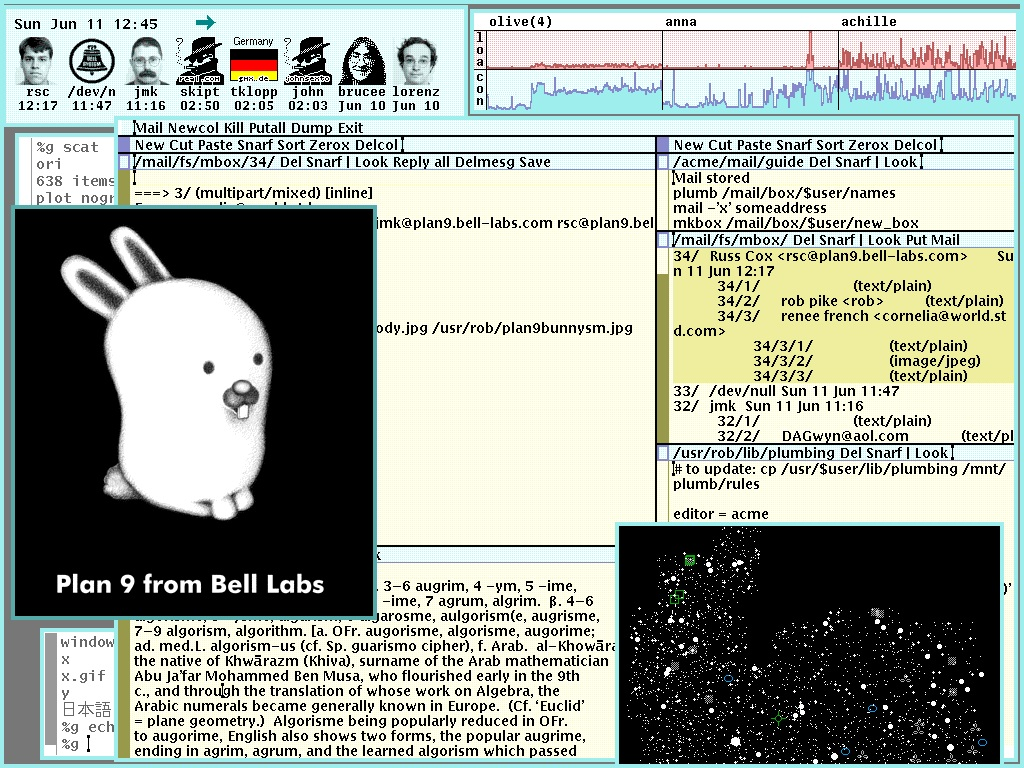
\includegraphics[width=0.9\linewidth]{screenshot.jpg}
	\caption{Plan 9 典型桌面截图（来源：官方 wiki）}
	\label{fig:screenshot}
\end{figure}

一段包含 JPEG 图片的多部分 MIME 邮件刚刚到达；该邮件的结构显示在右侧的 Acme 邮件目录中。截图中的主要组件包括：

\begin{itemize}
\item \textbf{faces(1)} —— 邮件通知程序，在有新邮件到达时显示提示。
\item \textbf{stats(8)} —— 系统状态监视器，实时显示 CPU、内存等资源使用情况。
\item \textbf{acme(1)} —— 集编辑、文件管理和程序执行为一体的开发环境。Acme 正在运行 Mail，它使用了邮件文件系统 upas/fs(4)。Acme 同时也在编辑\texttt{plumber(4)} 的规则文件。
\item \textbf{scat(7)} —— 星空目录浏览器，可交互式查看天文星表。
\item \textbf{page(1)} —— 图像查看器，正在显示 Plan 9 的吉祥物 Glenda。
\item \textbf{rio(1)} —— Plan 9 的窗口系统，负责管理所有窗口的布局和鼠标交互。
\end{itemize}

\section{工具背后的设计理念}

这些工具并非简单的应用程序，它们都深度融入了 Plan 9 的核心哲学：

\begin{enumerate}
\item \textbf{一切皆是文件}：\texttt{upas/fs(4)} 邮件文件系统将邮件消息和附件呈现为目录和文件，因此 Acme 可以直接浏览邮件结构，就像浏览本地文件一样。\texttt{plumber(4)} 的规则也是通过文件进行配置和动态加载的。
\item \textbf{9P 协议}：所有上述工具（包括窗口系统 rio）都通过 9P 协议与内核或其他服务通信。例如，Acme 通过 9P 挂载了邮件文件系统，从而能够透明地访问邮件内容。
\item \textbf{私有命名空间}：每个进程（如 acme 的各个窗口）都可以拥有独立的命名空间，这使得不同任务可以拥有不同的文件视图，互不干扰。
\item \textbf{Plumbing 机制}：\texttt{plumber} 作为程序间的通信枢纽，允许用户通过点击或拖拽将数据（如文本、图像、URL）从一个程序传递到另一个程序，极大地提高了工作效率。
\end{enumerate}

\section{学习启示}

对初学者而言，这个截图展示了 Plan 9 作为完整工作环境的实际面貌。建议在学习过程中尝试亲自运行这些工具，观察它们如何通过文件和协议协同工作。通过实践，您将更深刻地理解 Plan 9 为何被设计为“分布式系统的统一界面”，而不仅仅是一个操作系统内核。

屏幕截图的更多示例可以在官方 wiki 上找到，它们都是理解 Plan 9 使用方式的绝佳素材。
	
\chapter{核心概念：命名空间与 9P 协议}

命名空间和 9P 协议是 Plan 9 最为核心的两个概念，也是理解整个系统的钥匙。本章将深入剖析这两个相互支撑的机制：命名空间如何为每个进程提供私有的文件视图，通过 bind、mount、union 等命令实现灵活定制；9P 协议如何作为内核唯一识别的通信语言，将所有资源访问统一为标准的消息传递。

理解这两个概念，就等于理解了 Plan 9 与 Unix 的根本区别所在。本章内容较为抽象，但它是后续所有章节的基础，建议反复阅读并配合实际操作进行验证。
	
\section{命名空间（Namespace）}

\begin{itemize}
\item 命名空间是进程私有的文件视图，通过 \texttt{bind}、\texttt{mount}、\texttt{union} 等命令修改。
\item 联合挂载（Union Mounts）允许将多个目录合并为一个视图。
\item 使用 \texttt{namespace} 命令可查看当前命名空间配置。
\item 命名空间是实现进程隔离和沙盒化的基础。
\item 在 Plan 9 中，命名空间突变包括挂载一个到 9P 文件服务器的连接的能力。该连接可以是网络连接、管道或任何其他可读写的文件描述符。
\end{itemize}
	
\section{9P 协议基础}

\begin{itemize}
\item 9P2000（又称 Styx）是 Plan 9 第四版引入的协议版本，定义了 17 种基本消息类型。
\item \textbf{T-message}（请求）与 \textbf{R-message}（回复）机制，\texttt{fid}（文件标识符）用于跟踪打开的文件。
\item 9P 是内核唯一识别的协议，所有系统调用最终都转换为 9P 消息。
\item \textbf{典型应用实例}：acme、rio、plumber、ftpfs（FTP 客户端）、wikifs（维基编辑工具）、webfs（URL 数据检索）均以 9P 文件服务器形式实现。
\end{itemize}
	
% ============================================================
% 第二卷：用户空间与开发环境
% ============================================================

\part{用户空间与开发环境}
	
\chapter{rc Shell 与日常使用}

rc 是 Plan 9 的命令行解释器，它继承了 Unix shell 的基本功能，但在语法设计上更加简洁、规则更加统一。本章将系统讲解 rc 的语法精髓——命令分隔、后台执行、退出状态、模式匹配等核心特性。

此外，本章还将介绍 Plan 9 环境下的文本处理工具（正则表达式、sort、grep、awk）、进程管理（创建、信号、睡眠与唤醒）以及基本的网络操作。掌握 rc 是高效使用 Plan 9 的前提，也是后续进行系统管理和编程开发的基础。
	
\section{rc 语法精髓}

\begin{itemize}
\item 命令分隔符：\texttt{\&}（后台执行，进程 ID 存入 \texttt{\$apid}）和 \texttt{;}（顺序执行）。
\item 退出状态存入 \texttt{\$status} 变量。
\item 长命令行可用反斜杠 \texttt{\textbackslash} 续行。
\item 注释符 \texttt{\#}（引号内除外）。
\item 模式匹配：\texttt{*}（任意字符序列）、\texttt{?}（单字符）、\texttt{[class]}（字符类）。
\end{itemize}

\section{文本处理与系统管理}

\begin{itemize}
\item 正则表达式、排序与搜索（sort、grep）、awk 数据处理。
\item 进程管理：进程创建、进程组、信号（notes）、睡眠与唤醒。
\item 网络操作：网络连接与命名、服务提供、分布式计算基础。
\end{itemize}
	
\chapter{Acme 开发环境与编辑器}

Acme 不仅是文本编辑器，更是集编辑、文件管理、程序执行和用户界面于一体的综合开发环境。本章将深入介绍 Acme 的交互方式——三键鼠标的语义设计（左键选择、中键执行、右键搜索/获取）、Tag line（蓝色标签行）中的内置命令（Del、Snarf、Get、Look、Put），以及如何通过 namespace 查看 Acme 服务注册情况。

理解 Acme 的设计哲学，有助于体会 Plan 9“工具协同”的理念——编辑器不仅编辑文本，更是与系统其他部分交互的枢纽。

\section{三键鼠标语义}

\begin{itemize}
\item \textbf{Button 1（左键）}：选择文本、设置插入点。
\item \textbf{Button 2（中键）}：执行选中的命令。
\item \textbf{Button 3（右键）}：获取/打开选中内容，或执行搜索。
\end{itemize}
	
\section{Tag line 与内置命令}

Tag line（蓝色标签行）显示窗口路径，包含以下内置命令：

\begin{itemize}
\item \texttt{Del}：删除当前窗口
\item \texttt{Snarf}：复制选中文本到剪贴板
\item \texttt{Get}：加载文件
\item \texttt{Look}：搜索字符串
\item \texttt{Put}：保存文件
\end{itemize}

可通过 \texttt{namespace} 命令查看 Acme 服务注册情况。
	
\chapter{应用编程：C 语言与工具链}

Plan 9 的 C 编程环境自成体系。本章将带领读者从 Hello World 开始，逐步掌握使用 mk 构建系统、利用 rfork 进行进程控制、通过锁和交会实现并发同步、使用 Acid 调试器进行程序调试，以及编写合成文件服务器将服务呈现为文件系统。

本章是 Plan 9 应用开发的入门指南，也是后续深入内核编程的前置准备。建议读者在阅读本章时，同步在 Plan 9 环境中编写和运行示例代码。

\section{构建系统 \texttt{mk}}

\begin{itemize}
\item \texttt{mk} 是 Plan 9 的构建工具，替代 make，使用 Mkfile 编写构建规则。
\item 参考论文：《Maintaining Files on Plan 9 with Mk》—— Andrew G. Hume 和 Bob Flandrena。
\end{itemize}

\section{进程与并发}

\begin{itemize}
\item 进程创建：\texttt{fork}、\texttt{rfork}（细粒度共享/隔离控制）。
\item 同步机制：锁、队列锁、交会（rendezvous）。
\item 多线程编程与竞争条件处理。
\end{itemize}

\section{调试与合成文件服务器}

\begin{itemize}
\item \textbf{Acid 调试器}：基于语言构建的调试器，支持脚本化调试。
\item \textbf{服务构建}：编写扁平/层次化/动态合成文件服务器（如 ramfs、Clone 文件服务器）。
\end{itemize}

\chapter{图形与窗口系统深度}

Plan 9 的图形系统以简洁和统一著称。本章将深入其图形模型——Raster Graphics 的实现原理、Porter/Duff 图像合成算法、rio 窗口系统的定制方法（壁纸、颜色、鼠标键盘绑定），以及 Tom Duff 编写的 Panel 图形界面库的使用。

对于有兴趣进行图形界面开发的读者，本章提供了从原理到实践的完整路径。

\section{图形模型}

\begin{itemize}
\item Plan 9 的 Raster Graphics 实现。
\item Porter/Duff 图形合成模型。
\end{itemize}

\section{Rio 定制}

\begin{itemize}
\item 添加壁纸、修改颜色方案。
\item 鼠标与键盘绑定配置。
\end{itemize}

\section{Panel 库}

由 Tom Duff 编写的图形界面库，被 Mothra 网络浏览器等应用使用。参考：《A Quick Introduction to the Panel Library》。

\chapter{编程环境与工具链深度}
	
本章是对第五篇“应用编程”的深化与补充。我们将聚焦于 Plan 9 C 编译器（Ken Thompson 设计）的内部机制、APE（ANSI/POSIX Environment）跨平台移植环境的使用方法、Plan 9 汇编器的独特语法风格，以及系统对 Unicode 字符集的完整支持机制。

这些内容对于需要将外部软件移植到 Plan 9、或希望深入理解 Plan 9 工具链设计的开发者尤为重要。
	
\section{C 编译器与 APE}

\begin{itemize}
\item Plan 9 C 编译器由 Ken Thompson 设计，具有独特的代码生成与优化策略。
\item \textbf{APE（ANSI/POSIX Environment）}：用于在 Plan 9 与 Unix 之间移植 C 代码的环境。
\end{itemize}

\section{汇编器与字符集}
\begin{itemize}
\item Plan 9 汇编器具有独特的语法风格，详见《A Manual for the Plan 9 assembler》。
\item 完整的 Unicode 支持机制。
\end{itemize}
	
% ============================================================
% 第三卷：网络与分布式安全
% ============================================================

\part{网络与分布式安全}

\chapter{网络与分布式系统}

Plan 9 天生为分布式而设计。本章将介绍其网络架构——IL 协议的设计初衷与逐步淘汰的原因、TCP/IP 协议栈的实现、网络命名与连接管理机制，以及远程执行（cpu）、文件系统导入导出（import/exportfs）等分布式计算工具。

此外，本章还将介绍 9grid 网格计算基础设施、Drawterm 远程终端模拟器和 9VX 虚拟化方案，展示 Plan 9 如何将网络上的所有资源统一为可访问的文件。

\section{网络组织}

\begin{itemize}
\item IL 协议（轻量级传输协议）。
\item TCP/IP 协议栈支持。
\item 网络命名与连接管理。
\end{itemize}

\section{分布式计算}

\begin{itemize}
\item \texttt{cpu} 命令：远程执行程序。
\item \texttt{import} 与 \texttt{exportfs}：文件系统导入导出。
\item \textbf{9grid}：Plan 9 的网格计算基础设施。
\item \textbf{Drawterm}：Plan 9 终端模拟器，可从其他系统连接 Plan 9 环境。
\item \textbf{9VX}：Plan 9 虚拟化方案。
\end{itemize}

\chapter{9P 协议深度剖析}

9P 是 Plan 9 的“系统总线”。本章在前文 9P 基础之上，进一步深入协议的技术细节：消息的完整类型与结构、版本协商流程、fid 句柄的生命周期管理，以及 9P 在 Linux（v9fs）、macOS（Mac9P）、Unix（u9fs）等平台的跨生态实现。

理解 9P 的底层机制，是理解 Plan 9 一切设计的终点，也是为 Plan 9 开发新服务或驱动的前提。

\section{协议本质}

9P 是内核唯一识别的协议，所有系统调用（文件读写、设备访问、网络操作）均被转换为 9P 消息在客户端与服务器之间传递。

\section{消息机制深度}

\begin{itemize}
\item 版本协商、文件读写、属性查询的具体消息包结构。
\item \texttt{fid}（32 位句柄）由客户端选择，用于跟踪打开的文件和目录。
\end{itemize}

\section{跨平台生态}

\begin{itemize}
\item \textbf{Unix}：u9fs 服务器
\item \textbf{macOS}：Mac9P 客户端内核扩展
\item \textbf{Linux}：v9fs 驱动程序
\item \textbf{9pfuse}：FUSE 实现，可在非 Plan 9 系统上挂载 9P 文件系统
\end{itemize}

\chapter{Factotum 与安全架构深度}

Plan 9 的安全模型以 Factotum 认证代理为核心。本章将深入讲解 Factotum 用户级文件系统（/mnt/factotum）的密钥管理方式、支持的认证协议族（p9any、p9sk1/p9sk2、apop、cram、chap、rsa、pass），以及完整的客户端-服务器双向认证流程。

本章内容对于理解 Plan 9 如何在分布式环境中实现安全单点登录（SSO）至关重要，也是系统管理员和安全研究者的必备知识。

\section{Factotum 认证代理}

Factotum 是一个用户级文件系统（挂载于 /mnt/factotum），作为用户的认证代理，管理一组由 \texttt{attribute=value} 对构成的密钥。

\section{支持的认证协议}

\begin{itemize}
	\item \textbf{p9any}：元协议，用于协商实际使用的协议
	\item \textbf{p9sk1/p9sk2}：Plan 9 共享密钥协议及其变体
	\item \textbf{apop}、\textbf{cram}：POP3/IMAP 质询/响应协议
	\item \textbf{chap}：PPP/PPTP 质询/响应协议
	\item \textbf{rsa}：RSA 公钥解密，用于 SSH 和 TLS
	\item \textbf{pass}：明文密码
\end{itemize}

\section{认证流程}

客户端通过 Factotum 保管的秘密信息配合加密协议向服务器证明身份，部分协议支持双向认证。Factotum 可为任何拥有相同用户 ID 的进程充当客户端代理。

% ============================================================
% 第四卷：内核与存储系统
% ============================================================

\part{内核与存储系统}

\chapter{内核深入}

Plan 9 内核以简洁和可读性著称。本章将带领读者进入内核源码目录树（/sys/src/9/port、/sys/src/9/platform、/sys/src/9/ip），解析 conf 内核配置文件中 dev、ip、link、misc 等配置项的含义，并深入内存管理（KZERO 布局、虚拟内存映射）、进程调度（kproc、睡眠与唤醒）以及用户态设备驱动的开发方法。

本章适合具备一定操作系统基础知识的读者，是通往内核贡献者的必经之路。

\section{源码结构}

\begin{itemize}
\item \texttt{/sys/src/9/port}：可移植内核代码
\item \texttt{/sys/src/9/platform}：平台相关代码（如 pc、alphapc、ppc、iPAQ）
\item \texttt{/sys/src/9/ip}：IP 协议栈实现
\end{itemize}

\section{内核配置（conf 文件）}

\begin{itemize}
\item \textbf{dev}：设备驱动
\item \textbf{ip}：IP 协议（原生内核）
\item \textbf{link}：硬件特定驱动部分
\item \textbf{misc}：架构特定文件（VGA、SCSI 接口）
\item \textbf{lib}：内核链接库
\item \textbf{boot}：引导配置
\item \textbf{bootdir}：引导目录文件列表
\end{itemize}

\section{内存、进程与驱动}

\begin{itemize}
\item 内存管理：KZERO 布局、虚拟内存映射。
\item 进程调度：\texttt{kproc} 创建内核进程、睡眠与唤醒机制、共享内存多处理器支持。
\item \textbf{用户态设备驱动}：支持在用户空间调试驱动，调试完成后加载到内核以获得性能优势。
\end{itemize}

\chapter{高级文件系统与存储}

Plan 9 的存储体系以 Fossil 文件服务器和 Venti 归档存储为核心。本章将系统讲解 Fossil 的三层目录结构（/active、/snapshot、/archive）、Venti 基于 SHA1 哈希的去重块存储机制（log 与 index 架构）、访问控制模型（noworld 与 write 组），以及其他辅助文件系统（cwfs、hjfs、ramfs、unionfs、9pfs）。

理解这套存储体系，有助于把握 Plan 9 在数据持久化和版本管理方面的独特优势。

\section{Fossil 文件服务器}

Fossil 是 Plan 9 的主文件系统，运行在用户空间，作为磁盘写缓冲区，并可选择以 Venti 服务器作为归档存储后端。

\begin{itemize}
\item \textbf{/active}：常规文件系统根目录
\item \textbf{/snapshot}：临时快照（格式：/snapshot/yyyy/mmdd/hhmm）
\item \textbf{/archive}：长期快照（格式：/archive/yyyy/mmdds），存放在 Venti 服务器上
\end{itemize}

\section{Venti 归档存储}

\begin{itemize}
\item 基于 SHA1 哈希的去重块存储。
\item 存储分为日志（log）和索引（index）两部分。
\item 日志被分割为固定大小（如 500MB）的块。
\end{itemize}

\section{访问控制与其他文件系统}

\begin{itemize}
\item \textbf{访问控制}：默认要求认证票据；特殊组 \texttt{noworld}（权限削弱）和 \texttt{write}（只读限制）。
\item \textbf{其他文件系统}：cwfs、hjfs、ramfs（动态合成）、unionfs（深度联合）、9pfs（分布式文件系统）。
\end{itemize}

% ============================================================
% 第五卷：语言、商业化与生态对比
% ============================================================

\part{语言、商业化与生态对比}

\chapter{Alef 与并发先驱}

Alef 是 Plan 9 第二版引入的并发编程语言，由 Phil Winterbottom 设计。本章将介绍 Alef 的 C 风格语法、轻量级进程（任务）和通道通信机制，并追溯其并发模型对后续语言的深远影响——从 Alef 到 Inferno 的 Limbo，再到 Go 语言的 goroutine 与 channel。

了解这段语言谱系，有助于理解 Plan 9 在并发编程思想上的原创性贡献。

\section{Alef 语言}

由 Phil Winterbottom 设计，C 风格语法，内置轻量级进程（任务）和通道通信机制，是 Plan 9 第二版引入的并发编程语言。

\section{历史传承}

Alef 的并发模型 $\to$ Inferno 的 Limbo 语言 $\to$ Go 语言的 goroutine 与 channel，构成了贝尔实验室并发编程思想的完整谱系。

\chapter{Inferno 与 Limbo 语言}

Inferno 是 Plan 9 的姐妹操作系统，设计为可在裸硬件或多种宿主操作系统上运行。本章将介绍 Inferno 的架构设计，以及其核心编程语言 Limbo——一种类型安全的并发语言，编译为 Dis 虚拟机字节码执行。

对于希望探索 Plan 9 思想在更广泛平台上的应用的读者，本章提供了重要的延伸视角。

\section{Inferno 操作系统}
Plan 9 的姐妹系统，设计为可在裸硬件上运行，也可托管在其他操作系统之上，强调可移植性。

\section{Limbo 语言}

\begin{itemize}
\item 类型安全的并发语言。
\item 编译为 Dis 虚拟机字节码执行。
\item 所有用户态代码（除 shell 脚本外）均用 Limbo 编写。
\item 参考：《A Descent into Limbo》—— Brian W. Kernighan。
\end{itemize}

\chapter{商业化与衍生}

Plan 9 虽然主要作为研究系统，但其设计理念已展现出商业价值。本章将介绍最著名的商业化案例——Vita Nuova 公司对 Inferno 的持续维护和推广，以及 Plan 9 架构在嵌入式系统、分布式存储和网络设备等领域的应用场景。

了解商业化实践，有助于认识 Plan 9 思想在现实世界中的生命力。

\section{Vita Nuova 与 Inferno 的商业化}

一批公司成功销售了基于 Plan 9 的产品。最著名的是 \textbf{Vita Nuova}，它持续维护和推广 \textbf{Inferno}——一个面向机顶盒和其他嵌入式设备的 Plan 9 衍生品。

\section{Plan 9 的商业应用}

虽然 Plan 9 主要作为研究系统，但其设计理念在嵌入式系统、分布式存储和网络设备领域具有商业价值。

\chapter{与其他系统的对比与集成}

将 Plan 9 置于更广阔的操作系统生态中加以审视，有助于加深对其设计选择的理解。本章将从多个维度进行对比：Plan 9 vs Unix/Linux（单一协议 vs 杂乱系统调用）、Plan 9 vs Inferno（内核级分布式 vs 虚拟机级可移植性），并介绍 plan9port、npe（POSIX 兼容层）、9pfuse 等跨平台集成工具。

本章适合希望将 Plan 9 理念与其他系统互通的开发者阅读。

\section{Plan 9 vs Unix/Linux}

\begin{itemize}
\item Plan 9 不是 Unix 的变体，而是旨在替代 Unix。
\item 单一协议（9P）vs 杂乱无章的系统调用接口。
\item 命名空间隔离 vs 全局文件系统树。
\end{itemize}

\section{Plan 9 vs Inferno}

\begin{itemize}
\item Plan 9：内核级分布式系统，运行于特定硬件。
\item Inferno：虚拟机级可移植性，可运行于多种宿主操作系统。
\end{itemize}

\section{跨平台集成工具}

\begin{itemize}
\item \textbf{plan9port}：Unix/Linux/macOS 上的 Plan 9 用户空间工具。
\item \textbf{npe}：POSIX 兼容层，用于移植 POSIX 软件到 Plan 9。
\item \textbf{9pfuse}：Linux FUSE 驱动，可挂载 9P 文件系统。
\end{itemize}

\chapter{相关生态与软件}

Plan 9 的现代生态正在持续丰富。本章将介绍活跃社区开发的新应用——git9（Git 实现）、xmpp、disco（Discord 客户端）、hell（Mastodon 客户端），多媒体工具 mpl 和 treason，协同绘图工具 whiteboardfs，以及 9front ports tree 中维护的大量应用程序移植。

同时，本章也客观讨论了 Plan 9 面临的移植挑战——特别是缺少完整功能 Web 浏览器的问题，以及 webfs(4) 和 html(2) 作为解决方案的探索。

\section{现代应用}

本页面列出了为 Plan 9 编写或移植到 Plan 9 的主要软件包。更多用户贡献的软件托管在 Plan 9 文件服务器 sources.cs.bell-labs.com 的 /n/sources/contrib/ 目录下。

\begin{itemize}
\item \textbf{9pm}：适用于 Windows 的 Sam 及其他第二版 Plan 9 工具的移植版本。
\item \textbf{CVS 1.11.1p1}：CVS 1.11.1p1，从 CVS 仓库编译而来，移植到 Plan 9 。
\item \textbf{Graphviz}：适用于 Plan 9 的 Graphviz。
\item \textbf{GCC for Plan 9}：GCC，移植到 Plan 9。包含三个压缩包：二进制文件、APE 源代码和 GNU 源代码。
\item \textbf{Perl 5.8.0}：Perl 5.8.0，移植到 Plan 9。
\item \textbf{PQ}：PQ 数据库程序。
\item \textbf{Python 2.2+}：Python 2.2 以上版本，从 CVS 编译而来，移植到 Plan 9。
\item \textbf{Sun Sources}：适用于 Sun 工作站的第二版 Plan 9 源代码。对于有精力将 Sparc 内核更新到第四版的人来说很有用。Charles Forsyth 将第二版移植到 LX/Classic 的版本在此处http://www.caldo.demon.co.uk/plan9/dist/lx.tgz。
\item \textbf{TeX, Web2C v7.2}：TeX 和 LaTeX 文档排版系统，移植到 Plan 9。
\item \textbf{X11}：您真的不会想用这个。它又旧又慢，而且只在 8 位显示器上表现良好。
\item \textbf{git9}：Git 实现
\item \textbf{xmpp}：XMPP 客户端
\item \textbf{disco}：Discord 客户端
\item \textbf{hell}：Mastodon 客户端
\end{itemize}

\section{多媒体与协作}

\begin{itemize}
\item \textbf{mpl}：音乐播放器
\item \textbf{treason}：视频播放器
\item \textbf{whiteboardfs}：协同绘图文件系统
\end{itemize}

\section{9front Ports Tree}

9front 维护的大量应用程序移植，可通过 ports 树获取。

\section{移植挑战}

由于 Plan 9 具有与其它现代操作系统截然不同的系统模型，将外部软件移植到 Plan 9 有时会很困难。尤其是，Plan 9 没有功能完整的 Web 浏览器；\texttt{webfs(4)} 和 \texttt{html(2)} 被设计为迈向解决方案的步骤。

% ============================================================
% 第六卷：高阶实践与未来
% ============================================================

\part{高阶实践、调优与未来}

\chapter{特殊硬件与虚拟化}

Plan 9 的移植能力超出了 x86 平台。本章将介绍 Raspberry Pi（Richard Miller 移植）、Marvell Sheevaplug、Compulab Trimslice 等嵌入式与 ARM 平台上的运行方案，以及 QEMU、VirtualBox、9VX 等虚拟化方案和 Google Compute Engine（GCE）云平台的支持。

对于希望在非传统硬件上体验 Plan 9 的读者，本章提供了实用的操作指南。

\section{嵌入式与 ARM 平台}

\begin{itemize}
\item Raspberry Pi 上的 Plan 9 / 9front（Richard Miller 移植）。
\item Marvell Sheevaplug、Compulab Trimslice 等设备支持。
\item SDF Plan 9 Boot Camp。
\end{itemize}

\section{虚拟化与云平台}

\begin{itemize}
\item QEMU、VirtualBox 上的 Plan 9。
\item 9VX 虚拟化方案。
\item Google Compute Engine（GCE）虚拟磁盘镜像。
\end{itemize}

\chapter{Plan 9 与云计算/容器}

Plan 9 本质上是一个分布式操作系统，其“将网络上一切资源当作文件”的理念与云计算天然契合。本章将探讨 Plan 9 即云的思想、9P 协议在 NixOS 等容器化系统中的应用，以及 9P 作为容器间文件系统通信协议的潜力。

本章适合对云原生和容器技术感兴趣的读者，提供了一个从 Plan 9 视角审视现代基础设施的独特角度。

\section{Plan 9 即云}
Plan 9 本质上是一个分布式操作系统，将网络上的一切资源当作文件使用，这本身就是云的概念。

\section{9P 在容器化中的应用}

\begin{itemize}
\item NixOS 使用 9P 挂载存储目录。
\item 9P 可作为容器间文件系统通信协议。
\end{itemize}

\chapter{性能调优与系统管理}

将 Plan 9 用于实际工作环境时，性能调优和系统管理是必不可少的技能。本章将介绍系统监控工具（进程与资源监控、网络性能分析）、存储调优方法（Fossil 缓存配置、Venti 索引结构优化），以及常见故障的诊断与排查技巧。

本章内容对于 Plan 9 系统管理员和长期使用者具有直接的实用价值。

\section{系统监控}

进程与资源监控工具、网络性能分析。

\section{存储调优}

\begin{itemize}
\item Fossil 缓存配置优化。
\item Venti 索引结构调优。
\end{itemize}

\section{故障排查}

常见问题诊断、日志分析、系统恢复技巧。

\chapter{项目创意与贡献实践}

参与 Plan 9 社区开发是提升技能、回馈社区的重要途径。本章将列举适合 Google Summer of Code 的项目方向（窗口管理器、设备驱动、网络协议、文件系统、GUI 应用），介绍使用 Patch 工具的贡献流程，并分享参与 9fans 邮件列表、IRC 频道等社区交流的经验和建议。

本章鼓励读者从学习者转变为贡献者，并保持开放心态拥抱 Plan 9 的独特概念。

\section{适合 GSoC 的项目方向}

\begin{itemize}
\item 新的窗口管理器
\item 设备驱动开发
\item 网络协议实现
\item 文件系统服务构建
\item 图形界面应用
\end{itemize}

\section{贡献流程与社区参与}

\begin{itemize}
\item 使用 Patch 工具提交代码。
\item 参与 9fans 邮件列表、Freenode IRC（\#plan9）、9front 社区。
\item 保持开放心态，拥抱不同于 Unix 的独特概念。
\end{itemize}

\chapter{社区生态与持续发展}

Plan 9 不仅是一个操作系统，更是一个充满活力的社区。本章将介绍 9front 分支的现代活力（月度更新、Wi-Fi/音频/USB 支持、amd64/arm64 镜像）、文档工作组（Documentation Task Force）的持续努力，以及 9social 等社区项目的创新实践。

最后，本章回顾了 sources.cs.bell-labs.com 每日更新机制，展望 Plan 9 未来的发展方向，并鼓励读者参与社区建设。

\section{9front 的现代活力}

\begin{itemize}
\item 月度更新，持续增加 Wi-Fi、音频、USB、内置模拟器等现代硬件支持。
\item 提供 amd64 和 arm64 的 QEMU 镜像。
\end{itemize}

\section{文档工作组与社区项目}

\begin{itemize}
\item Plan 9 文档工作组（Documentation Task Force）持续修复和更新文档。
\item \textbf{9social}：基于 git 和纯文本文件的去中心化社交网络，有 Plan 9/9front 客户端实现。
\item 任何拥有 Plan 9 安装的人都可以编辑 wiki 页面。
\end{itemize}

\section{日常开发与更新}

Plan 9 至今仍通过 \texttt{sources.cs.bell-labs.com} 每日更新。这些变化被分发给众多 Plan 9 用户。sources 的每日快照通过其 dump 文件系统提供便捷的发布历史。

\chapter{吉祥物 Glenda —— Plan 9 的文化符号}

技术之外，Plan 9 也有其温暖的一面。本章介绍吉祥物 Glenda 的诞生故事，以及 Glenda 所象征的思索、简洁、友善的 Plan 9 精神。

了解这些文化符号，有助于读者更好地融入这个独特的技术社区。

\section{Glenda 的诞生}

Glenda 是 Plan 9 操作系统的官方吉祥物，由艺术家 Renée French 绘制，很快就成为 Plan 9 社区最亲切的文化象征。

\begin{figure}[htbp]
	\centering
	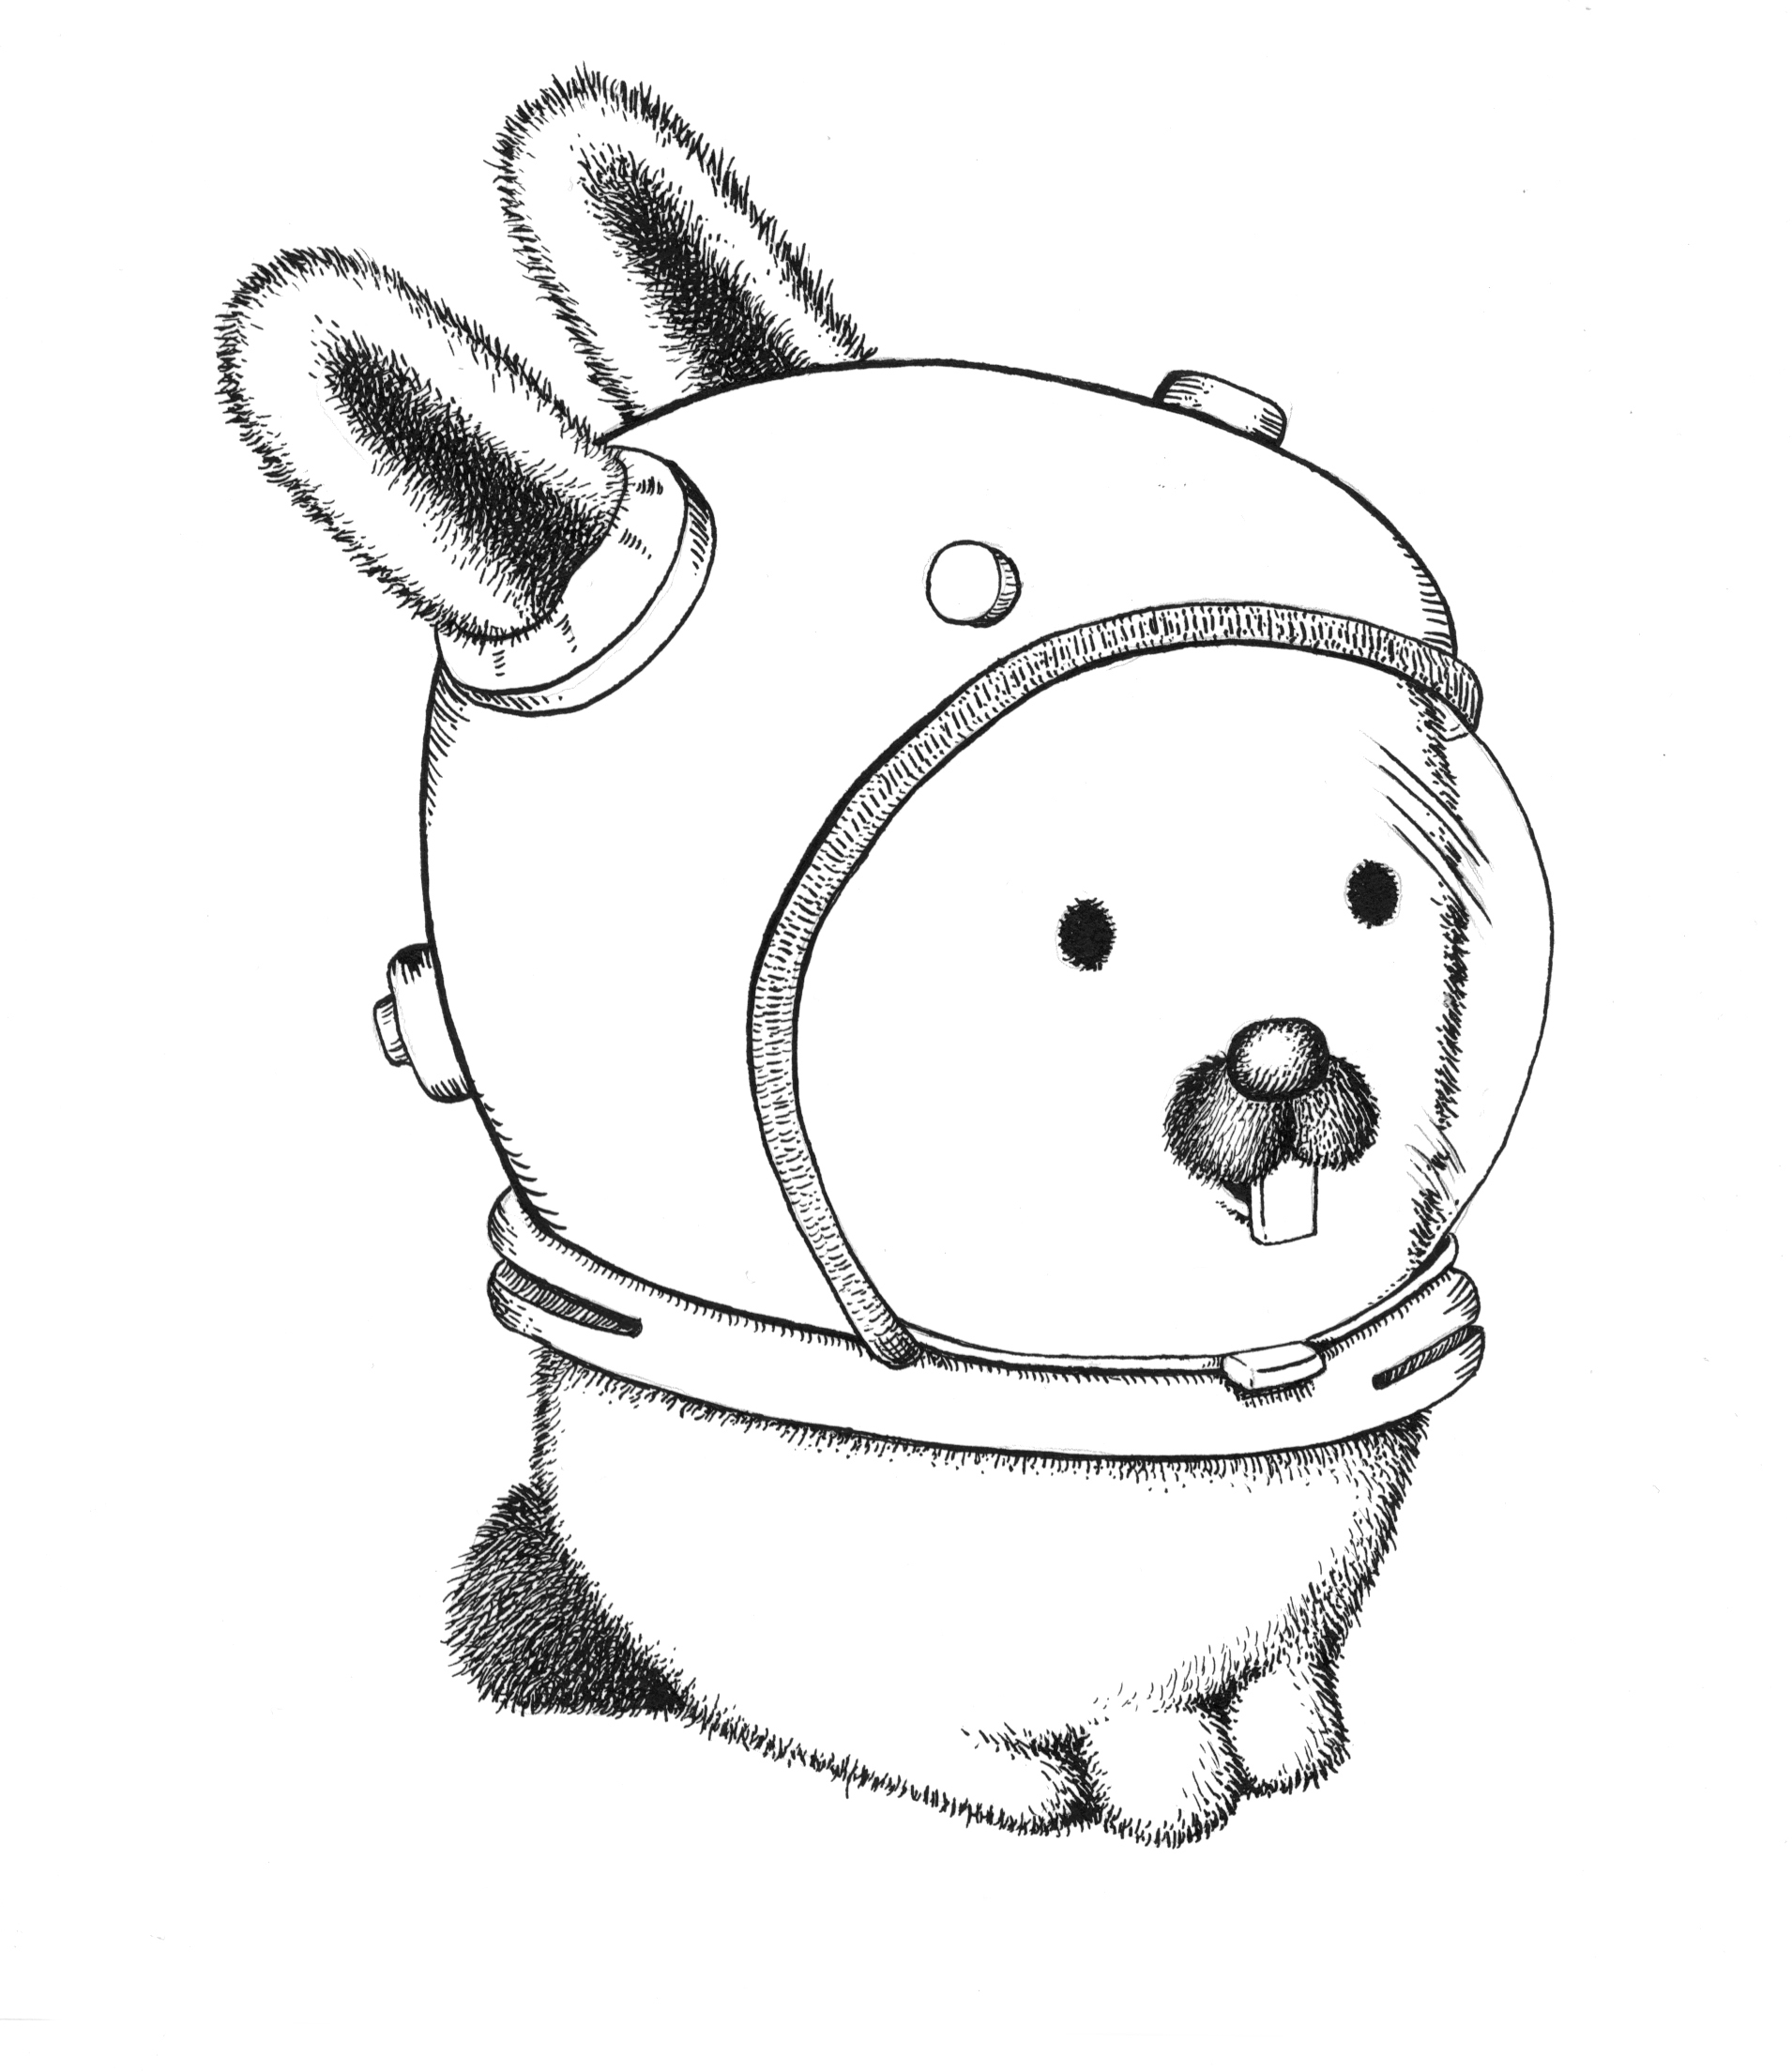
\includegraphics[width=0.6\linewidth]{spaceglenda300.jpg}
	\caption{Glenda}
	\label{fig:glenda_white}
\end{figure}

当需要更高分辨率的版本时，Renée French 绘制了一幅更大的画作，经扫描和调整后，生成了两个版本：白底版和黑底版。

\begin{figure}[htbp]
	\centering
	
\includegraphics[width=0.6\linewidth]{plan9bunnywhite.jpg}
	\caption{Glenda 白底版（高分辨率 JPEG）}
	\label{fig:glenda_white}
\end{figure}

\begin{figure}[htbp]
	\centering
	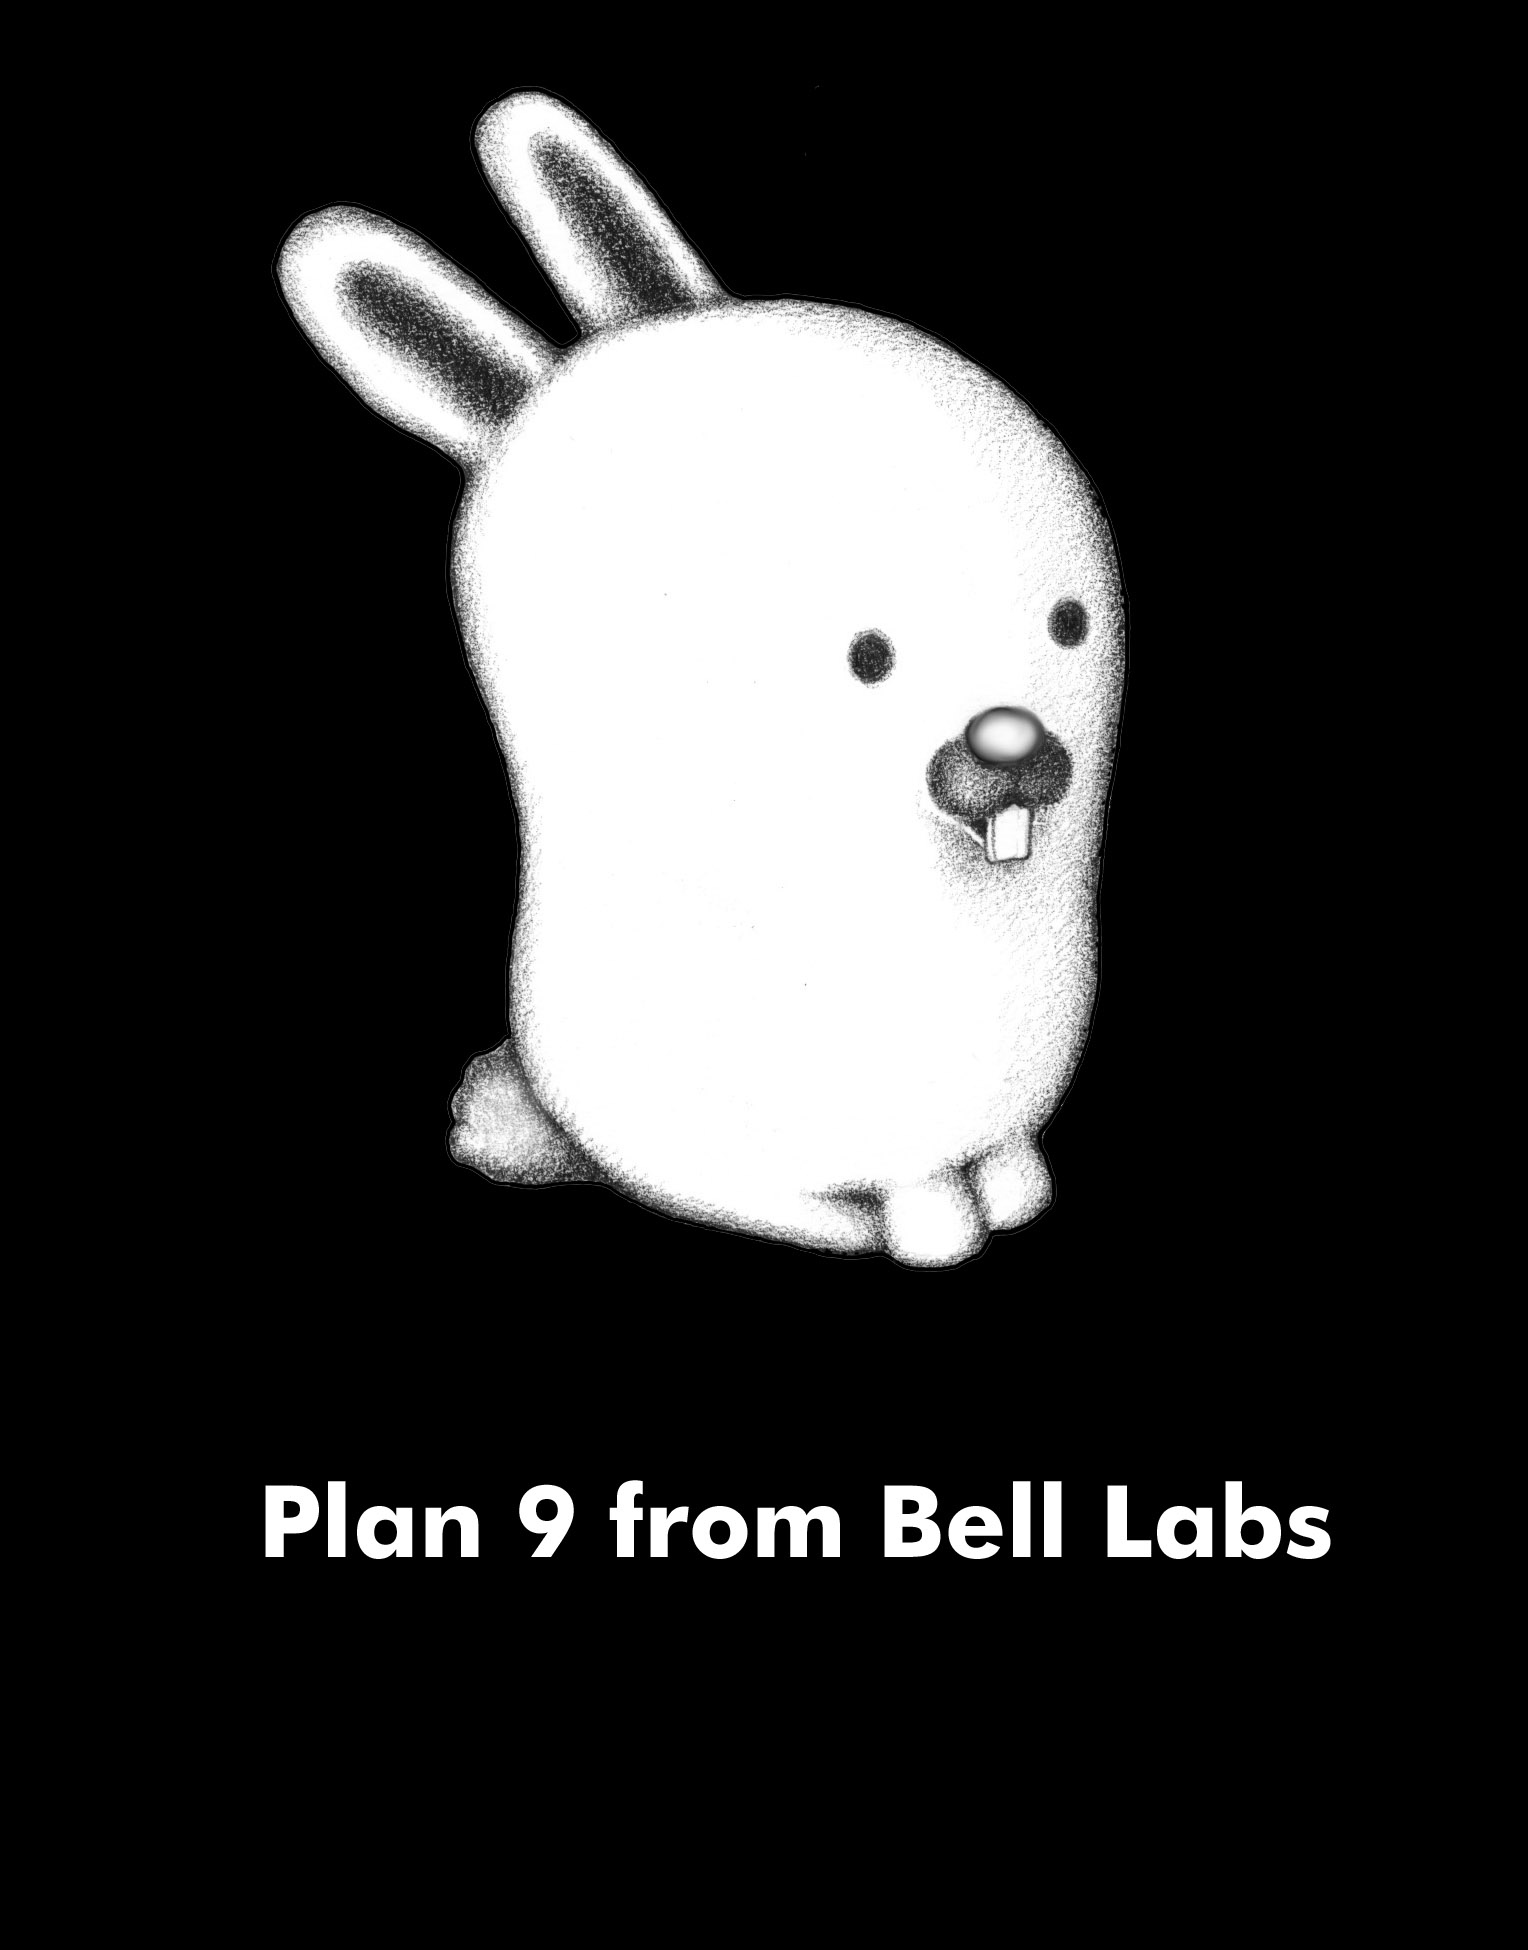
\includegraphics[width=0.6\linewidth]{plan9bunnyblack.jpg}
	\caption{Glenda 黑底版（高分辨率 JPEG）}
	\label{fig:glenda_black}
\end{figure}

高分辨率 JPEG 版本可通过点击官方网站上的对应图片获取。

\section{使用许可与社区传统}
Plan 9 社区鼓励大家使用这些图像制作 T 恤、贴纸和其他周边产品。这是一种深厚的社区传统，也是对 Plan 9 精神的致敬。
	
\begin{shuming}
	\textit{“Feel free to use these images to make t-shirts and other paraphernalia, but if you do a production run, please send us a sample for our collection.”}
\end{shuming}

如果您批量制作了相关周边，欢迎寄送一份样品给开发团队，作为收藏。这种开放、分享的精神，正是 Plan 9 社区长久以来保持活力的重要原因。

\section{Glenda 的意义}
Glenda 不仅是一个可爱的卡通形象，更代表着 Plan 9 的设计哲学：
\begin{itemize}
	\item \textbf{思索}——她手持圆规，象征对系统架构的深思熟虑。
	\item \textbf{简洁}——她的线条简单，却充满个性，如同 Plan 9 的代码一样精炼。
	\item \textbf{友善}——她欢迎所有好奇的学习者，鼓励探索和实验。
\end{itemize}

在您学习 Plan 9 的旅程中，Glenda 将是一个温暖的陪伴。许多社区聚会、讲座和文档中都会出现她的身影。了解她的故事，也是融入这个独特社区的入口之一。

% ============================================================
% 附录
% ============================================================
\backmatter

\chapter*{附录 A：核心论文与文献汇总}

\begin{center}
	\begin{tabular}{|c|c|c|}
		\hline
		\textbf{论文标题} & \textbf{作者} & \textbf{核心主题} \\
		\hline
		Plan 9 from Bell Labs & Rob Pike 等 & 系统总览（必读） \\
		The Use of Name Spaces in Plan 9 & Rob Pike 等 & 命名空间机制 \\
		The Organization of Networks in Plan 9 & Dave Presotto 等 & 网络架构 \\
		Security in Plan 9 & Russ Cox 等 & 安全与 Factotum \\
		How to Use the Plan 9 C Compiler & Rob Pike & C 编程入门 \\
		Acid: A Debugger Built From A Language & Phil Winterbottom & 调试器设计 \\
		Maintaining Files on Plan 9 with Mk & Andrew G. Hume 等 & Mk 构建工具 \\
		8½, the Plan 9 Window System & Rob Pike & 窗口系统 \\
		Rc — The Plan 9 Shell & Tom Duff & rc Shell 设计 \\
		Acme: A User Interface for Programmers & Rob Pike & Acme 环境 \\
		Venti: A new approach to archival storage & Sean Quinlan 等 & Venti 去重存储 \\
		The Plan 9 File Server & Ken Thompson & 文件服务器实现 \\
		The ALEF users guide & Bob Flandrena & Alef 语言 \\
		A Descent into Limbo & Brian W. Kernighan & Limbo 语言 \\
		\hline
	\end{tabular}
\end{center}

\chapter*{附录 B：版本历史时间线}

\begin{center}
	\begin{longtable}{|c|p{8cm}|}
		\hline
		\textbf{年份} & \textbf{事件} \\
		\hline
		1980 年代末 & Plan 9 项目启动 \\
		1992 & 第一版发布（仅限大学） \\
		1995 & 第二版发布（书+CD，\$350） \\
		1999 & Brazil 项目恢复名为 Plan 9 \\
		2000 年 6 月 & 第三版发布（免费互联网分发） \\
		2000--2001 & 9P2000 协议开发 \\
		2002 & 第四版发布（Lucent Public License 1.02） \\
		2003 年初 & Fossil 文件服务器首次亮相 \\
		2021 年 3 月 & MIT License 发布 \\
		\hline
	\end{longtable}
\end{center}

\chapter*{附录 C：历史版本下载与校验信息}

所有历史版本的 Plan 9 均已根据 MIT 许可证的条款重新发布。下表列出了从第一版到第四版（含最终版）的所有 ISO 和 tar 包下载链接。

\section*{版本下载链接}

\begin{center}
\begin{longtable}{|c|c|c|}
\hline
\textbf{版本} & \textbf{美国镜像} & \textbf{法国镜像} \\
\hline
第一版 & \href{https://9p.io/releases/1st/plan9-1st.iso}{ISO} / \href{https://9p.io/releases/1st/plan9-1st.tar}{tar} & \href{https://9p.io/france/releases/1st/plan9-1st.iso}{ISO} / \href{https://9p.io/france/releases/1st/plan9-1st.tar}{tar} \\
第二版 & \href{https://9p.io/releases/2nd/plan9-2nd.iso}{ISO} / \href{https://9p.io/releases/2nd/plan9-2nd.tar}{tar} & \href{https://9p.io/france/releases/2nd/plan9-2nd.iso}{ISO} / \href{https://9p.io/france/releases/2nd/plan9-2nd.tar}{tar} \\
第三版 & \href{https://9p.io/releases/3rd/plan9-3rd.iso}{ISO} / \href{https://9p.io/releases/3rd/plan9-3rd.tar}{tar} & \href{https://9p.io/france/releases/3rd/plan9-3rd.iso}{ISO} / \href{https://9p.io/france/releases/3rd/plan9-3rd.tar}{tar} \\
第四版（初始版） & \href{https://9p.io/releases/4th/plan9-4th.iso}{ISO} / \href{https://9p.io/releases/4th/plan9-4th.tar}{tar} & \href{https://9p.io/france/releases/4th/plan9-4th.iso}{ISO} / \href{https://9p.io/france/releases/4th/plan9-4th.tar}{tar} \\
第四版（最终版） & \href{https://9p.io/releases/4th/plan9-4th-final.iso}{ISO} / \href{https://9p.io/releases/4th/plan9-4th-final.tar}{tar} & \href{https://9p.io/france/releases/4th/plan9-4th-final.iso}{ISO} / \href{https://9p.io/france/releases/4th/plan9-4th-final.tar}{tar} \\
\hline
\end{longtable}
\end{center}

\section*{校验信息}
所有版本的 SHA1 校验和可在以下地址获取：
\begin{center}
	\url{https://9p.io/releases/sha1sums}
\end{center}

\section*{说明}
\begin{itemize}
	\item 上表中的两个第四版分别代表：初始发布版本，以及贝尔实验室在持续更新和修补后提供的最终版本。
	\item 所有历史版本均已根据 MIT 许可证条款重新发布。
	\item 美国镜像与法国镜像内容相同，可根据网络情况选择较快的源。
\end{itemize}

这些历史版本对于深入理解 Plan 9 的演进过程具有重要价值。建议学习者在阅读本框架的同时，结合不同版本的实际体验，感受系统设计思想的变迁。

\chapter*{附录 D：社区资源与入口}

\begin{itemize}
	\item 官方网站：\url{https://plan9.io}
	\item 活跃分支 9front：\url{http://9front.org}
	\item 在线手册：\url{http://man.cat-v.org/9front/}
	\item 社区维基与学习笔记：\url{https://github.com/EdoardoLaGreca/9knowledge}
	\item IRC：\#plan9 on Freenode / \#9front on OFTC
	\item 邮件列表：9fans
	\item 国际 Plan 9 研讨会（IWP9）
	\item 源代码服务器：\texttt{sources.cs.bell-labs.com}
\end{itemize}
	
\end{document}